\ifx\allfiles\undefined

	% 如果有这一部分另外的package,在这里加上
	% 没有的话不需要
	
	\begin{document}
\else
\fi
    \chapter{目标规划}
    目前已介绍的线性规划、运输规划、整数规划问题中,只涉及单一优化目标,即只有一个目标函数:
    \begin{itemize}
        \item 利润最大
        \item 成本最小
        \item 质量最好
        \item 时间最短
        \item ……
    \end{itemize}
而在现实问题中,往往需要考虑多种要求(不相兼容的,“鱼与熊掌不可兼得”或多个目标)多个目标间是不同的、矛盾的、甚至
。此时,上述方法难以凑效。美国学者Charnes和Coope,1961年提出目标规划方法,用来处理多目标决策问题。\\
    \section{目标规划问题}
    \begin{dfnbox}{目标规划}{amznotes}
        \textbf{目标规划} 是多目标优化的一种主要方法。
    \end{dfnbox}
    \textbf{主要思想:}目标规划在处理多目标决策问题时,并不是直接寻找满足这些目标的最优解,而是通过引入\textcolor{red}{“偏差变量”}将目标转化为\textcolor{red}{约束}处理,
    以\textcolor{red}{“各个目标的偏差量尽可能小”}为原则构造一个新的目标函数,继而求解基于这个新目标函数的单目标规划问题\footnote{本质上,目标规划在“寻求最大限度地满足所有目标的解”}。\\
    \textbf{目标规划与一般线性规划的区别}:
    \begin{enumerate}
        \item 能处理多个目标函数的最优问题
        \item 目标规划可在相互矛盾的约束条件下,找到满意解
        \item 目标规划找到的不是绝对的最优解,而是与“人为指定目标相比较”的相对最优解
        \item 目标规划对约束条件的处理不是“不分主次”,而是有“轻重缓急"
    \end{enumerate}
    \subsection{单目标的目标规划}
    \begin{exbox}{汽车制造利润问题}{}
        \textbf{例:}某汽车制造厂根据市场需求拟生产A,B,C三种型号的家用轿车.具体的相关数据如表6.1所示。
        生产线每天工作 8h,问该厂如何安排生产计划可使每月(按30天计)所获利润最大?
        \begin{table}[H]
            \centering
            \label{tab:6.1}
            \renewcommand{\arraystretch}{1.5}
            \begin{tabular}{|c|c|c|c|}
                \hline
                车型 & 工时 (h/辆) & 市场需求 (辆/月) & 利润 (万元/辆) \\ \hline
                A & 8  & 10  & 2.5  \\ \hline
                B & 10 & 15  & 3.5  \\ \hline
                C & 12 & 9   & 4    \\ \hline
            \end{tabular}
            \caption{相关数据}
        \end{table}
        \textbf{解:}
        
            设 \( x_i \)(\( i=1,2,3 \))分别表示 A、B、C 三种车型的生产数量,一个月正常生产工时为 240 小时,则问题可建模为:
        
            \[
            \text{max } z = 2.5x_1 + 3.5x_2 + 4x_3
            \]
            \[
            \text{s.t. }
            \begin{cases} 
                x_1 \leq 10, \\ 
                x_2 \leq 15, \\ 
                x_3 \leq 9, \\ 
                8x_1 + 10x_2 + 12x_3 \leq 240, \\ 
                x_i \geq 0 \text{ 且为整数} \quad (i=1,2,3).
            \end{cases}
            \]
            其中,\( 8x_1 + 10x_2 + 12x_3 \leq 240 \) 为每月总工时限制(式 5.1)。
        
            这是一个单目标整数规划模型,直接求解得最优解为 \( x_1^* = 2 \)、\( x_2^* = 14 \)、\( x_3^* = 7 \),最优值 \( z^* = 82 \)。即每月正常生产 A、B、C 型轿车分别为 2 辆、14 辆、7 辆,可获得最大利润 82 万元。
    \end{exbox}
    这道例题本身没什么意义,但是注意,上述的市场需求是根据以往的销售数据预测得到的结果,但实际中的销售情况未必就是这样,要充分考虑市场条件的变化和实际生产能力的限制条件等因素,来调整具体的生产方案。比如可能有下列情况出现:
    \begin{enumerate}
        \item 车型 B 销量可能下降,车型 C 可能上升,故应考虑 \( x_2 \leq x_3 \);
        \item 车型 A 原材料成本增加导致利润下降,应适当减少其产量;
        \item 尽量利用原有设备工时,避免加班生产;
        \item 尽可能达到或超过原利润指标 82 万元。
    \end{enumerate}
    综合考虑上述的几种情况,重新调整生产方案,即是多(4个)目标的决策问题了,这就是目标规划要解决的一类问题。不难注意到以上几个限制条件都会减少利润,因此如果加上这些条件后,利润还能达到甚至超过82万元是最好的,达不到的话,也应该尽量接近;因此我们想到定义偏差量$d^+$和$d^-$,用来衡量实际利润和预期指标值82万元的偏差。
    
    \begin{exbox}{续:用目标规划思想解决上例}{}
    \begin{itemize}
        \item \textbf{偏差量定义}
        
        实际利润与预期指标值82万元的偏差用$d^+$和$d^-$表示,其中:
        \begin{align*}
            d^+ &= \text{实际值} - \text{指标值} \quad (\text{超额完成}) \\
            d^- &= \text{指标值} - \text{实际值} \quad (\text{未完成})
        \end{align*}
        且规定$d^+, d^- \geq 0$。
    
        \item \textbf{偏差量性质}
        \begin{enumerate}
            \item 超额完成时:$d^+ > 0$,$d^- = 0$
            \item 未完成时:$d^+ = 0$,$d^- > 0$
            \item 恰好完成时:$d^+ = d^- = 0$
        \end{enumerate}
        由此可得:
        \[ d^+ \cdot d^- = 0 \]
    
        \item \textbf{目标函数转换}
        
        原目标函数:
        \[ \max z = 2.5x_1 + 3.5x_2 + 4x_3 \]
        可等价表示为:
        \[ 2.5x_1 + 3.5x_2 + 4x_3 + d^- - d^+ = 82 \]
        
        其中:
        \begin{itemize}
            \item 当$z > 82$时:$z - d^+ = 82$
            \item 当$z < 82$时:$z + d^- = 82$
        \end{itemize}
        也可将其视为一个约束条件(目标函数转化为约束条件)——在此称为\textcolor{red}{目标约束}(是软约束),模型中原来的约束条件称为\textcolor{red}{系统约束(绝对约束)}(是硬约束)。
    
        \item \textbf{目标规划模型}
        
        构造新的目标函数:
        \[ \min z = d^- - d^+ \]
        
        完整模型(6.1.3):
        \begin{align*}
            \text{min } & z = d^- - d^+ \\
            \text{s.t. } & 
            \begin{cases} 
                x_1 \leq 10, \\ 
                x_2 \leq 15, \\ 
                x_3 \leq 9, \\ 
                8x_1 + 10x_2 + 12x_3 \leq 240, \\
                \textcolor{red}{2.5x_1 + 3.5x_2 + 4x_3 + d^- - d^+ = 82}, \\
                d^+, d^- \geq 0, \quad x_i \geq 0 \quad (i=1,2,3)
            \end{cases}
        \end{align*}
        该目标规划模型(6.1.3)与原模型(6.1.2)完全等价。
    \end{itemize}
    \end{exbox}
    可以看到,我们通过引入偏差量,将原目标函数加入约束条件,用偏差量构建新的目标函数,这就是目标规划所在做的事情。原来的硬约束是必须满足的,但是由原目标函数“下沉”得到的约束条件是软约束,可以不符合,只是尽量满足。
    
    
    
    

    
    
    \subsection{多目标的目标规划}
    多目标的目标规划核心思想就是\textcolor{red}{将多目标转化为单目标},是通过\textcolor{red}{满意解}\footnote{面对有可能互相冲突的约束,只能协商让各方都能满意的解}而非绝对最优解。
    \begin{itemize}
        \item 多个目标函数的加权处理,得到单一目标函数,再进行单目标优化求解
        \begin{align*}
            \text{Max } Z_1 \\
            \text{Min } Z_2 & \quad \longrightarrow \quad \max \lambda_1 Z_1 - \lambda_2 Z_2 + \lambda_3 Z_3 \quad ; \lambda_1, \lambda_2, \lambda_3 \text{ 是加权系数}
        \end{align*}
        \item 在多个目标函数中选择并保留一个主目标函数,其他目标函数处理为“不低于”或“不高于”可接受的约束条件,从而化为单目标函数,再进行单目标优化求解
        \begin{align*}
            \text{Max } Z_1 \\
            \text{Min } Z_2 & \quad \longrightarrow \quad \max Z_3 \\
            \text{s.t.} \quad Z_1 & \geq \alpha_1 \\
            Z_2 & \leq \alpha_2 \\
            \alpha_1, \alpha_2 & \text{ 是可接受值}
        \end{align*}
        \item 目标规划
    \end{itemize}

\begin{exbox}{续:引入多目标}{}
    \textbf{多目标的目标规划}

当存在4个不同目标时,需要适当调整生产计划,同时尽量保证利润不减少。各目标及其数学表达如下:

\begin{enumerate}
    \item 尽可能达到或超过原计划利润指标82万元:
    \[ 2.5x_1 + 3.5x_2 + 4x_3 + d_1^- - d_1^+ = 82 \]
    
    \item 车型B的产量不应大于车型C的产量:
    \[ x_2 - x_3 + d_2^- - d_2^+ = 0 \]
    
    \item 车型A的原材料成本增加,应适当降低其产量:
    \[ x_1 + d_3^- - d_3^+ \leq 10 \]
    
    \item 尽量充分利用原有设备台时,避免加班生产:
    \[ 8x_1 + 10x_2 + 12x_3 + d_4^- - d_4^+ \leq 240 \]
\end{enumerate}

\noindent \textbf{优先因子设置}

由于四个目标通常无法同时满足,需设定优先等级(重要程度),并且规定$p_k>p_{k+1}$:
\begin{itemize}
    \item 第1位目标优先因子:$p_1$
    \item 第2位目标优先因子:$p_2$
    \item 第3位目标优先因子:$p_3$
    \item 第4位目标优先因子:$p_4$
\end{itemize}
其中满足$p_k \gg p_{k+1}$($k=1,2,3,4$)。

\noindent \textbf{目标规划模型}

综合上述目标,建立目标规划模型:
\[ \min z = p_1 d_1^+ + p_2 d_2^+ + p_3 d_3^+ + p_4 (d_4^+ + d_4^-) \]

约束条件:
\[
\begin{cases}
    x_1 \leq 10, \quad x_2 \leq 15, \quad x_3 \leq 9, \\
    2.5x_1 + 3.5x_2 + 4x_3 + d_1^- - d_1^+ = 82, \\
    x_2 - x_3 + d_2^- - d_2^+ = 0, \\
    x_1 + d_3^- - d_3^+ \leq 10, \\
    8x_1 + 10x_2 + 12x_3 + d_4^- - d_4^+ \leq 240, \\
    d_j^-, d_j^+ \geq 0 \quad (j=1,2,3,4), \\
    x_i \geq 0 \quad \text{且为整数} \quad (i=1,2,3).
\end{cases}
\]
(观察目标函数,优先级依次是:利润低于82万元的量尽可能少>车型B高于车型C的量尽可能少>车型A产量的超出量尽可能少>设备台时的利用尽可能充分、少加班)。
\end{exbox}

\section{目标规划的数学模型}
一般说来,对于任一个多目标决策问题,多个目标总能有主次之分,即可根据各个目标的主次排出优先等级。\\
\begin{itemize}
\item \textbf{不同优先级:}不妨设问题有$L(\geq1)$个目标,可分为$K(K\leq L)$个优先等级。排在第1位的目标赋予最高的优先因子$p_1$,第2位的赋予优先因子$p_2$,依此类推,第k位的赋予优先因子$p_k(k\geq1)$,且规定$p_k\geq p_{k+1},k=1,2,\cdots,k-1$。\\
\item \textbf{相同优先级:}如果要区别相同等级的两个目标,通过加权系数来决定其主次:如同一等级目标的偏差量$d_k^-$,$d_k^+$赋予加权系数$w_k^-$,$w_k^+$,这些都是根据实际问题来确定的。
\end{itemize}
给出多目标决策问题的一般的目标规划模型:
\begin{thmbox}{目标规划的数学模型}{}

    \[
    \min z = \sum_{k=1}^{k} p_k \left[ \sum_{l=1}^{L} \left( w_l d_l^+ + w_l d_l^- \right) \right]\footnote{这是目标规划下的,体现多目标的单目标目标函数形式}
    \]
    
    其中,$d_l^+$ 和 $d_l^-$ 是目标的偏差项,$w_l$ 是目标的权重。
    
    约束条件为:
    
    \[
    \sum_{j=1}^{n} c_{ij} x_j + d_l^+ - d_l^- = g_l \quad (l=1, 2, \dots, L)\footnote{这是由各个目标转化成的软约束}
    \]
    
    \[
    \sum_{j=1}^{n} a_{ij} x_j \leq(\geq,=)b_i \quad (i=1, 2, \dots, m)\footnote{这是所有硬约束,是多目标模型里原有的}
    \]
    
    \[
    x_j \geq 0 \quad (j=1, 2, \dots, n)
    \]
    
    \[
    d_l^+, d_l^- \geq 0 \quad (l=1, 2, \dots, L)
    \]
    
    其中,$c_{ij} \quad (j=1, 2, \dots, n; l=1, 2, \dots, L)$ 为各目标的相关参数;$g_l \quad (l=1, 2, \dots, L)$ 为第一个目标的指标值;$a_{ij}, b_i \quad (i=1, 2, \dots, m)$ 为系统约束的相关系数。
    
    \end{thmbox}
    \textbf{说明:}
    \begin{enumerate}
        \item 在由实际问题建立目标规划的数学模型时,对于目标的选择、优先等级和加权系数的确定一般都与决策者的\textcolor{red}{主观性}有关,因此,实际中可以采用专家评定法或相应的科学方法来决定;
        \item 由于目标约束是软约束,实际中\textcolor{red}{不一定要求绝对满足},因此,所得问题的解不一定是可行解,但是\textcolor{red}{满意解};
        \item 一般根据各目标的\textcolor{red}{具体要求}来确定新的目标函数,一般原则是:
        \begin{enumerate}
            \item 如果要求恰好达到目标值,即要求目标的正负偏差都尽可能小,则取\textcolor{red}{ $\min z=f (d_{k}^{+}+d_{k}^{-})$ };
            \item 如果要求超过指标值,即要求目标的正偏差不限,而负偏差越小越好,则取\textcolor{green}{$\min z=f (d_{k}^{-})$} ;
            \item 如果要求不超过指标值,即要求目标的负偏差不限,而正偏差越小越好,则取\textcolor{blue} {$\min z=f (d_{k}^{+})$};
        \end{enumerate}
        按照以上原则:
        \begin{itemize}
            \item 确定各目标的\textcolor{red}{目标函数};
            \item 再根据各目标的优先级子问题应\textcolor{red}{优先因子和加权系数}
            \item 最后构成目标函数的\textcolor{red}{最小化}问题。
        \end{itemize}
        \item 如果某个目标(如第 $k_0$ 个)不属于第 $k_0$ 优先等级,则在模型中相应的加权系数 $w_{k_0}$ 满足 $1 \le k_0 \le K, 1 \le l \le S$ \textcolor{red}{都为 0}。
    \end{enumerate}

    \section{目标规划的求解方法}
    \subsection{总体思路}
    \begin{notebox}{\textbf{总体思路}}{}
    \begin{itemize}
    \item \textbf{转化:}将多目标问题转换成单目标问题;
    \item \textbf{求解:}按照前几章学过的多种方法求解\footnote{从目标规划的数学模型结构来看,它与线性规划的数学模型结构没有什么本质的区別,所以可用单纯形法的思想来求解}。
    \end{itemize}
    \end{notebox}

    \subsection{序贯算法}
    \begin{figure}[H]
        \centering
        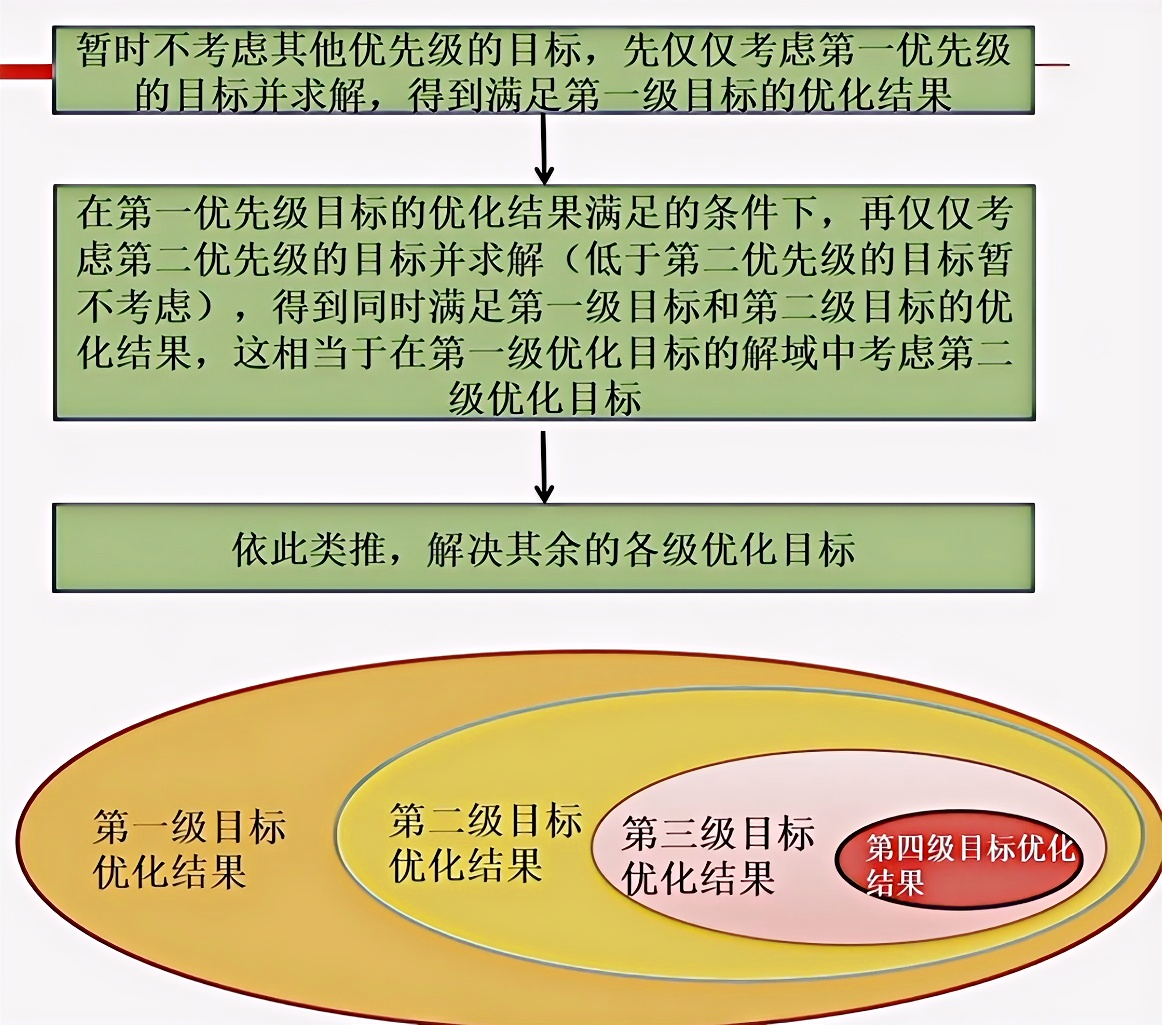
\includegraphics[width=0.46\textwidth]{./image/28.png}
        \caption{目标规划的序贯算法流程}
        \label{fig:Chapter4_Temporary_Pavilion_1}
    \end{figure}
    \section{案例分析}
    \begin{exbox}{VCD销售问题}{}
        \textbf{例:}某音像销售公司现有5名全职销售员和4名兼职销售员,全职销售员每月工作160h,
        兼职销售员每月工作80h。根据过去的销售记录,全职销售员平均每小时销售VCD25张,平均工资
        15元/h,加班工资22.5元/h。兼职销售员平均每小时销售VCD10张,平均工资10元/h,加班工资
        也是10元/h。现在预测下月VCD的销售量为27500张。公司每周营业6天,所以销售员可能需要加
        班才能完成任务,已知每出售一张 VCD 盈利 1.5元。公司经理认为,保持稳定的就业水平加上
        必要的加班,比不加班但就业水平不稳定要好,但全职销售员如果加班过多,就会因为疲劳过度而
        使得工作效率下降。因此,不允许每月加班超过100h,试建立数学模型分析研究该公司的工作安
        排方案。\\
        \textbf{解:}根据问题的实际情况,首先分析确定问题的目标及优先级:

        \begin{itemize}
            \item 最高优先级目标($p_1$):YCD销售量不少于27500张
            \item 第二优先级目标($p_2$):限制全职销售员加班时间不超过100h
            \item 第三优先级目标($p_3$):保持全体销售员的充分就业,加倍优先考虑全职销售员
            \item 第四优先级目标($p_4$):尽量减少销售员的加班时间,按利润贡献比例区分优先级
        \end{itemize}
        
        \noindent \textbf{1. 销售量目标约束}
        
        设$d_1^-$表示未达销售目标的偏差量,$d_1^+$表示超额完成的偏差量:
        
        \[
        \min z_1 = d_1^-
        \]
        \[
        \text{s.t. } 25x_1 + 10x_2 + d_1^- - d_1^+ = 27500
        \]
        
        \noindent \textbf{2. 工作时间目标约束}
        
        设$d_2^-, d_2^+$为全职销售员停工和加班偏差,$d_3^-, d_3^+$为兼职销售员偏差:
        
        \[
        \min z_2 = 2d_2^- + d_3^-
        \]
        \[
        \text{s.t. }
        \begin{cases}
        x_1 + d_2^- - d_2^+ = 5 \times 160, \\
        x_2 + d_3^- - d_3^+ = 4 \times 80.
        \end{cases}
        \]
        
        \noindent \textbf{3. 加班限制目标约束}
        
        设$d_4^-, d_4^+$为全职销售员加班时间偏差:
        
        \[
        \min z_3 = d_4^+
        \]
        \[
        \text{s.t. } x_1 + d_4^- - d_4^+ = 9 \times 100
        \]
        
        \noindent \textbf{4. 加权加班目标约束}
        
        根据利润贡献比(全职:兼职=3:1):
        
        \[
        \min z_4 = d_2^+ + 3d_3^+
        \]
        \[
        \text{s.t. }
        \begin{cases}
        x_1 + d_2^- - d_2^+ = 5 \times 160, \\
        x_2 + d_3^- - d_3^+ = 4 \times 80.
        \end{cases}
        \]
        
        \noindent \textbf{完整目标规划模型}
        
        \[
        \min z = p_1 d_1^- + p_2 d_4^+ + p_3 (2d_2^- + d_3^-) + p_4 (d_2^+ + 3d_3^+)
        \]
        \[
        \text{s.t. }
        \begin{cases}
        25x_1 + 10x_2 + d_1^- - d_1^+ = 27500, \\
        x_1 + d_2^- - d_2^+ = 5 \times 160, \\
        x_2 + d_3^- - d_3^+ = 4 \times 80, \\
        x_1 + d_4^- - d_4^+ = 9 \times 100, \\
        x_1, x_2, d_i^-, d_i^+ \geq 0 \quad (i=1,2,3,4).
        \end{cases}
        \]
    \end{exbox}
    
\ifx\allfiles\undefined
	% 如果有这一部分的参考文献的话,在这里加上
	% 没有的话不需要
	% 因此各个部分的参考文献可以分开放置
	% 也可以统一放在主文件末尾。
	
	%  bibfile.bib是放置参考文献的文件,可以用zotero导出。
	% \bibliography{bibfile}
	
	end{document}
	\else
	\fi